%**************************************************************************************
% License:
% CC BY-NC-SA 4.0 (http://creativecommons.org/licenses/by-nc-sa/4.0/)
%**************************************************************************************

\documentclass[notes]{beamer}

\mode<presentation> {

\usetheme{Madrid}

% Burnt orange
\definecolor{burntorange}{rgb}{0.8, 0.33, 0.0}
\colorlet{beamer@blendedblue}{burntorange}
% Pale yellow
\definecolor{paleyellow}{rgb}{1.0, 1.0, 0.953}
\setbeamercolor{background canvas}{bg=paleyellow}
% Secondary and tertiary palett
\setbeamercolor*{palette secondary}{use=structure,fg=white,bg=burntorange!80!black}
\setbeamercolor*{palette tertiary}{use=structure,fg=white,bg=burntorange!60!black}

% To remove the footer line in all slides uncomment this line
%\setbeamertemplate{footline}
% To replace the footer line in all slides with a simple slide count uncomment this line
%\setbeamertemplate{footline}[page number]

% To remove the navigation symbols from the bottom of all slides uncomment this line
%\setbeamertemplate{navigation symbols}{}
}

\usepackage{amsmath}
\usepackage{bm}
\usepackage{breqn}
\usepackage{graphicx} % for figures
\usepackage{subcaption} % for subplots 
\usepackage[labelsep=space,tableposition=top]{caption}
\renewcommand{\figurename}{Fig.} 
\usepackage{cleveref}
\usepackage{caption,subcaption}% http://ctan.org/pkg/{caption,subcaption}
\usepackage{booktabs} % Allows the use of \toprule, \midrule and \bottomrule in tables
\usepackage{multirow}

% To print 2 slides on a page
%\usepackage{handoutWithNotes}
%\pgfpagesuselayout{2 on 1}[border shrink=2mm]
%----------------------------------------------------------------------------------------
%	TITLE PAGE
%----------------------------------------------------------------------------------------
% The short title appears at the bottom of every slide, the full title is only on the title page
\title[CE394M: FEM Geo]{CE394M: FEM applied to Geotechnical Engineering} 
\author{Krishna Kumar} % name
\institute[UT Austin] % institution 
{
University of Texas at Austin \\
\medskip
\textit{
  \url{krishnak@utexas.edu}} % Your email address
}
\date{\today} % Date, can be changed to a custom date

\begin{document}

\begin{frame}
\titlepage % title page as the first slide
\end{frame}

\begin{frame}
 % Table of contents slide, comment this block out to remove it
 \frametitle{Overview}
 % Throughout your presentation, if you choose to use \section{} and \subsection{} 
 % commands, these %will automatically be printed on this slide as an overview 
 \tableofcontents
\end{frame}

%----------------------------------------------------------------------------------------
% slides
%----------------------------------------------------------------------------------------
\section{Nicoll Highway Collapse, Singapore}
%------------------------------------------------
\begin{frame}
\frametitle{Soil profile}
	\begin{figure}[ht]
		\centering
		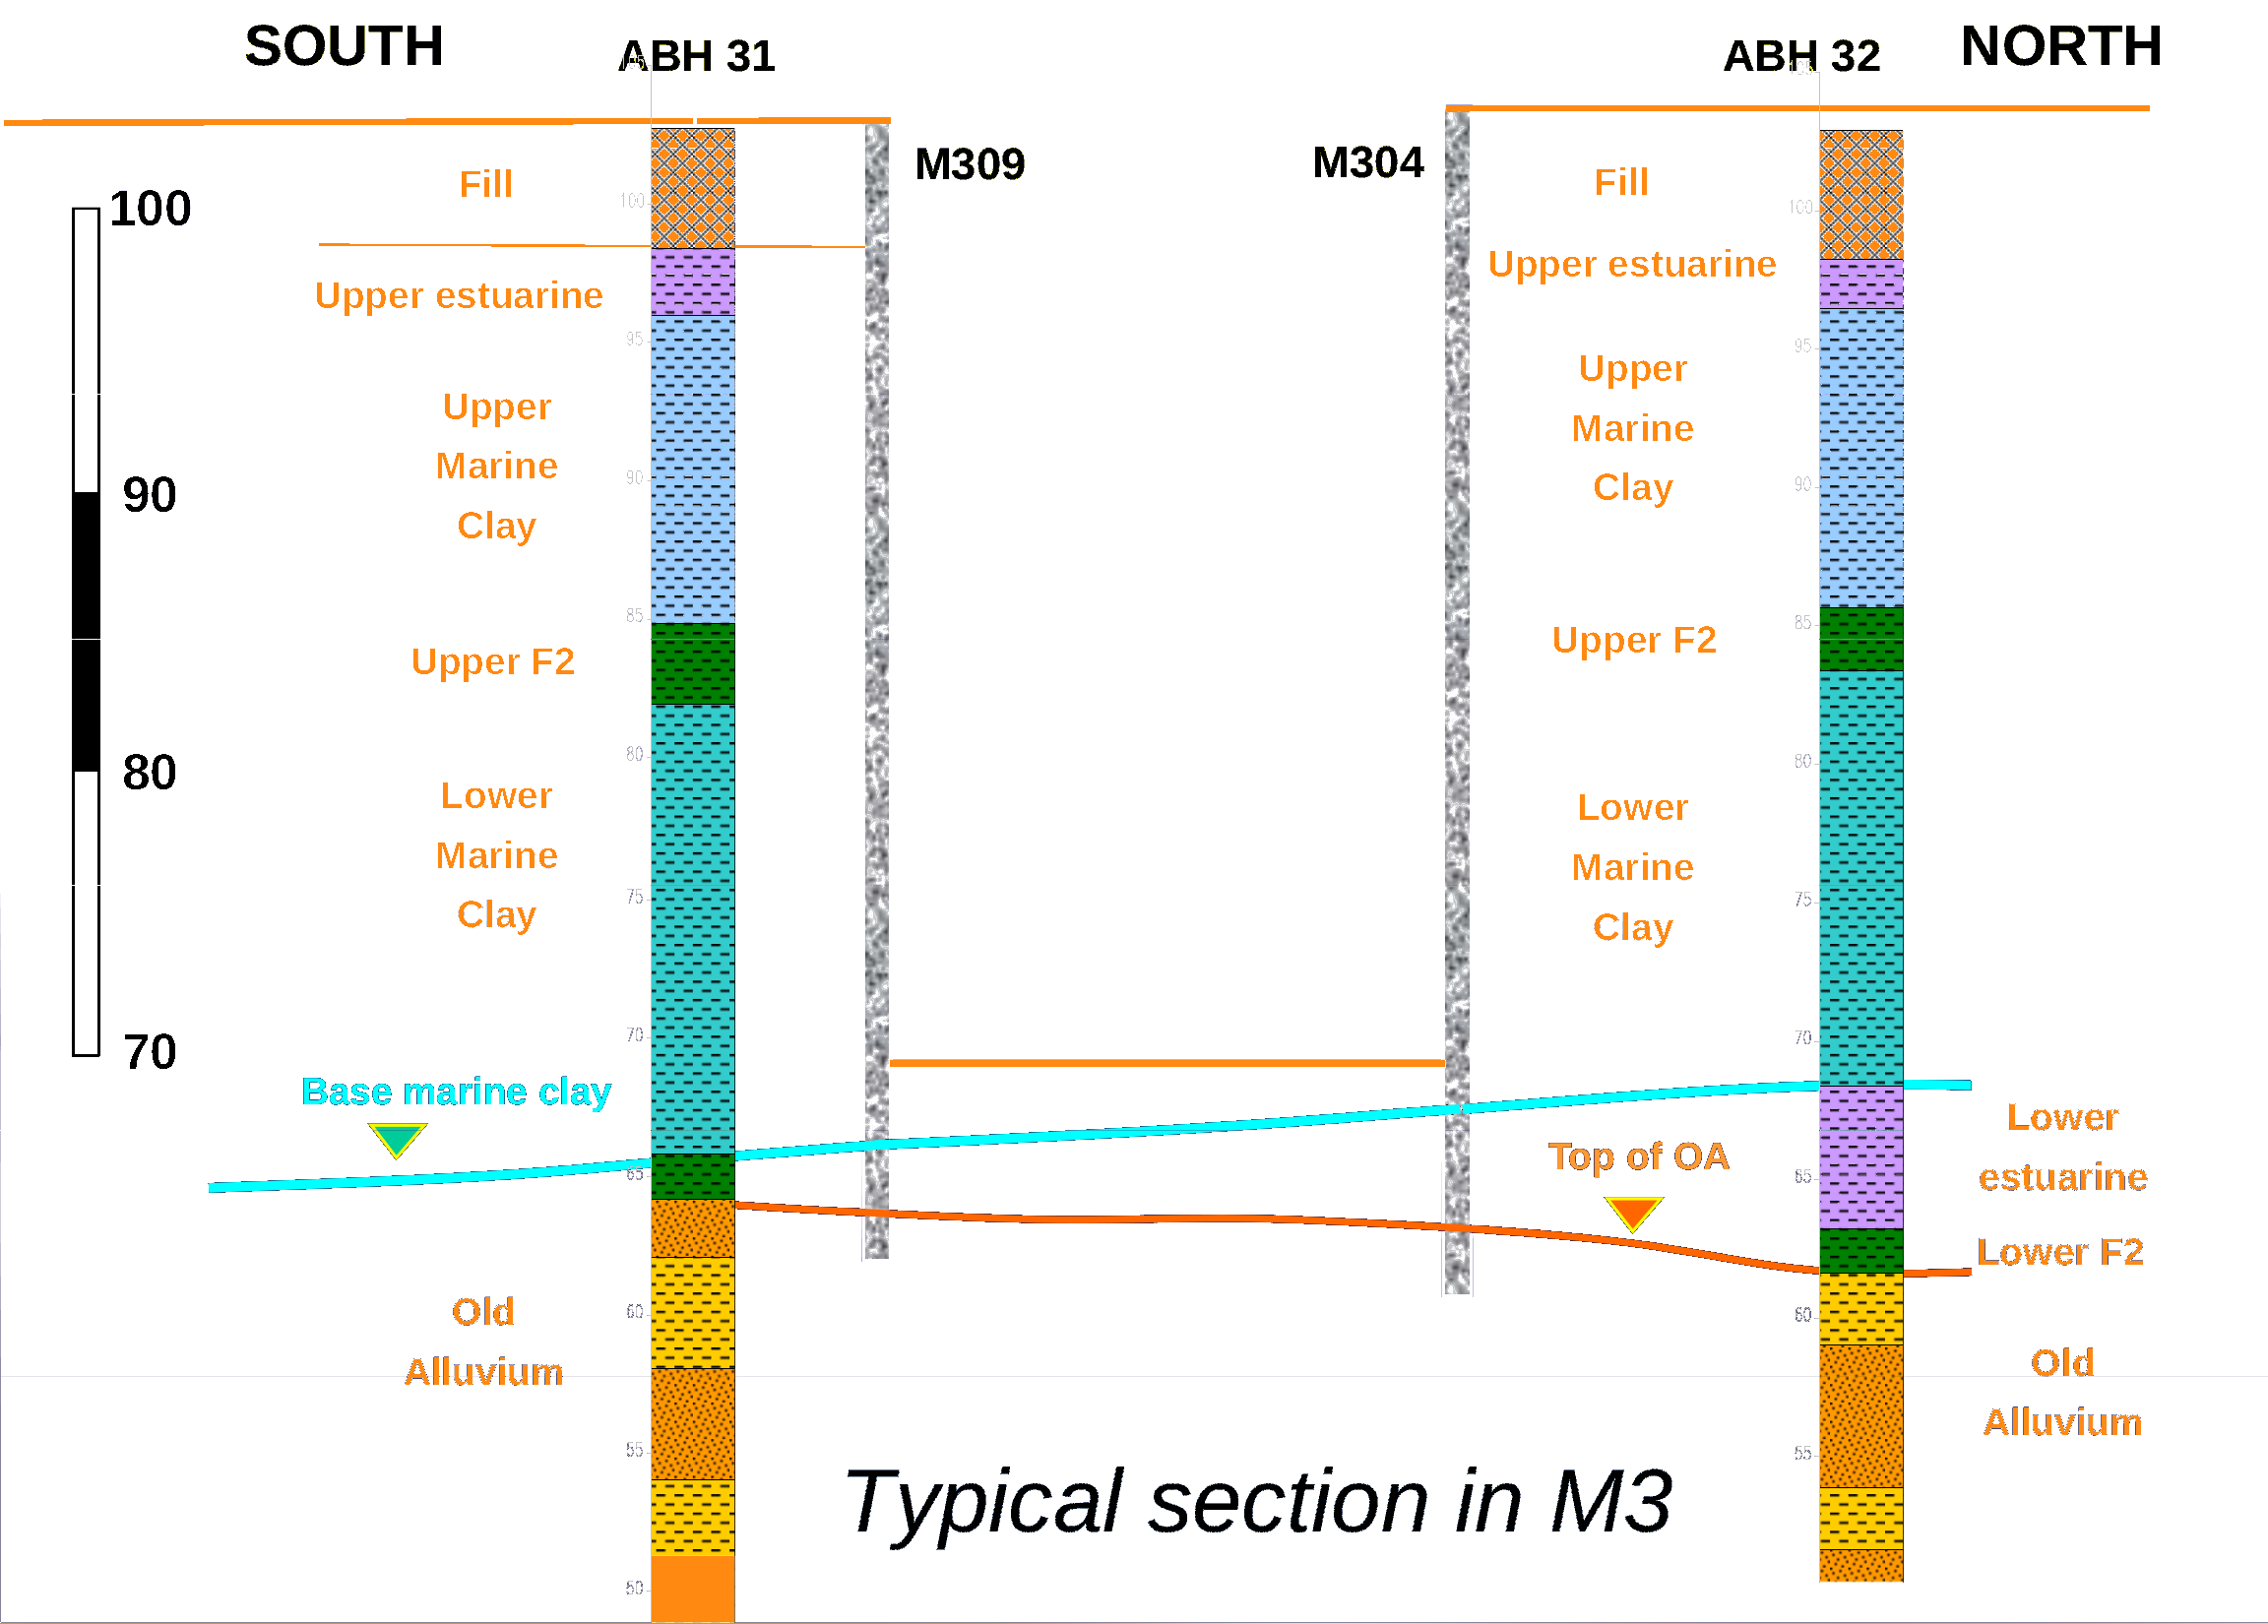
\includegraphics[width=0.85\textwidth]{figs/profile.png}
	\end{figure}
\end{frame}

%------------------------------------------------
\begin{frame}
\frametitle{Bending moments}
	\begin{figure}[ht]
		\centering
		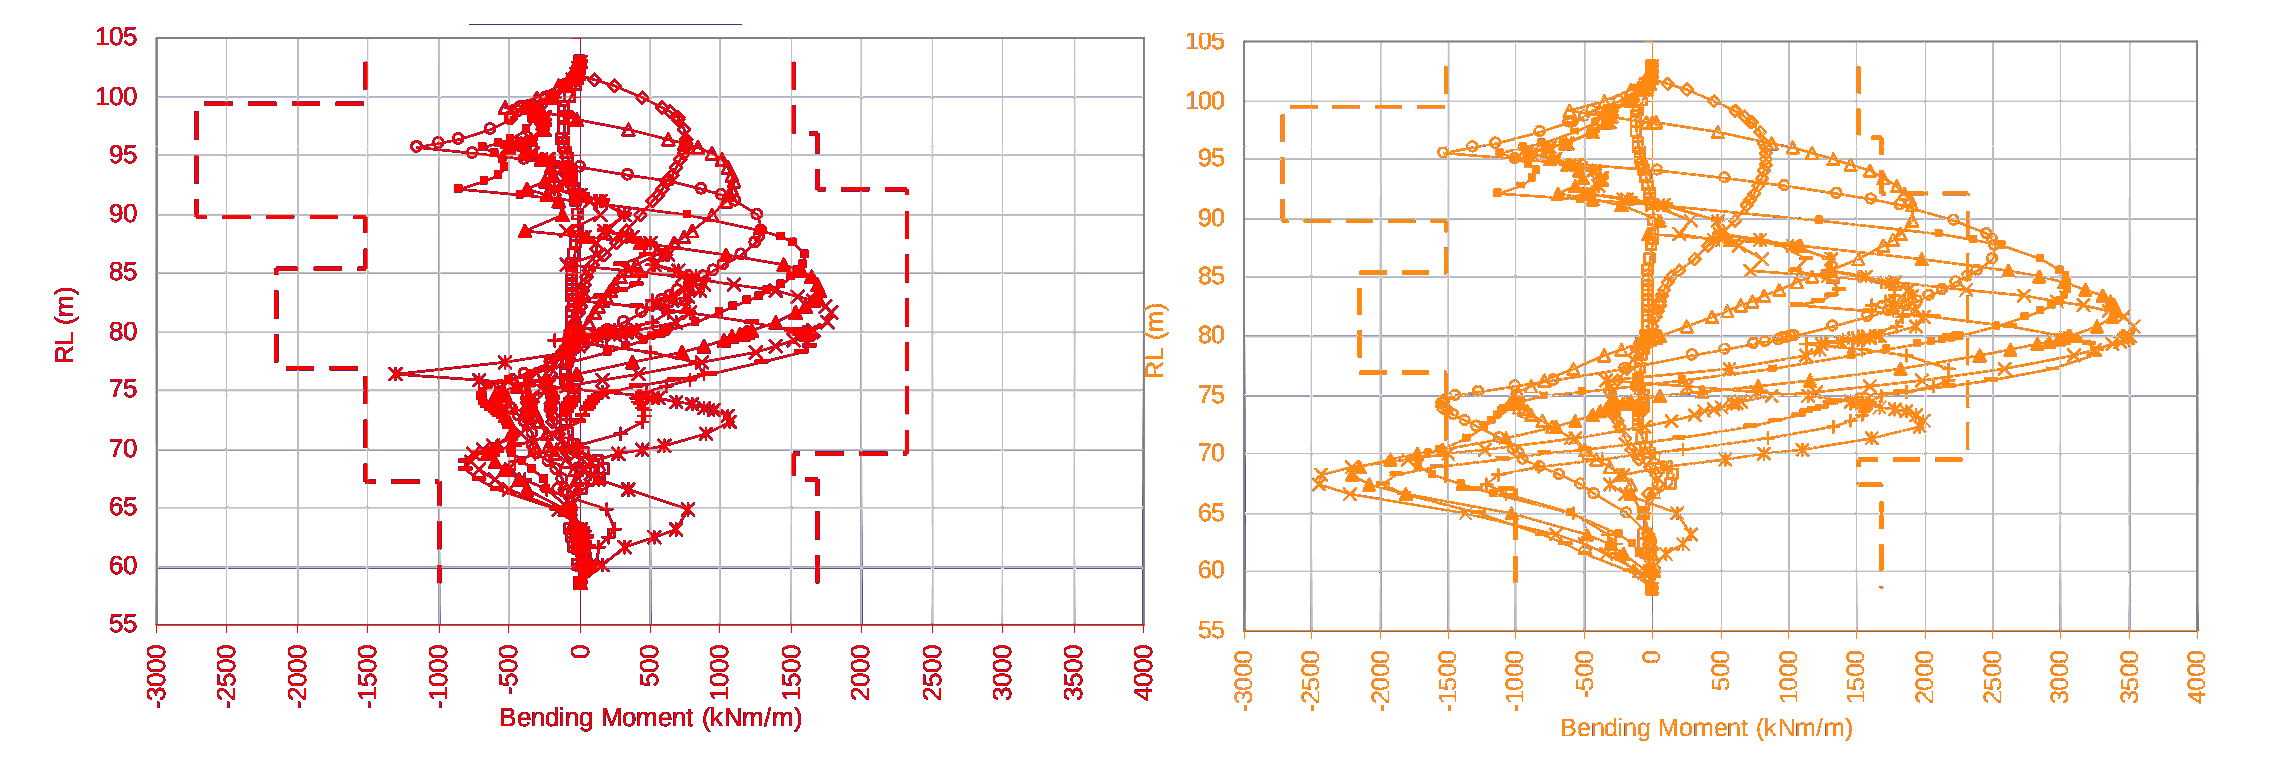
\includegraphics[width=\textwidth]{figs/bending-moments.png}
		\caption*{Method A vs Method B}
	\end{figure}
\end{frame}

\end{document}